Let $O$ be an optimal set and recall that we assume that $f(O) = 1$.
Let $T = \arg\max\{S, \displaystyle{\arg\max_{e \in U}}f(\{e\})\}$ 
be the set returned by the modified greedy algorithm, 
where $S$ is the set computed by the greedy algorithm~\ref{alg:greedy},
we prove the following theorem:

\begin{theorem}
$f(T) \geq (1 - e^{-1/2})$.
\end{theorem}

\begin{proof}
We can assume that $f(e) \leq 1 - e^{-1/2}$ for every $e \in U$ or otherwise the proof holds. 
Note, also, that if $|O \setminus T| \leq 1$ then $f(T) \geq 0.5$. 
Thus we assume the algorithm drops at least two elements from $O$ during its running. 
Denote by $x$ and $y$ the first and second such elements respectively.
Denote by $A$ the set of elements chosen by the algorithm just before dropping $x$ and by
$B$ the set of elements chosen right after dropping $x$ and before dropping $y$.
If $f(A) \geq 1 - e^{-1/2}$ the theorem holds, otherwise denote $f(A) = 1 - e^{-(1/2 - \delta)}$,
where $\delta$ might be in the range $(0, 0.5)$.  

We argue that the following inequalities hold:

\begin{align}
c(A) \leq 0.5 - \delta 
\\
c(x) > 0.5 + \delta
\\
c(O \setminus x) \leq 0.5 - \delta
\\
c(B) > 2\delta
\\
f(x) < 1 - e^{-1/2}
\\
\label{ineq:T}
f(O \setminus x | A) \geq e^{-1/2} - 1 + e^{-(1/2 - \delta)}
\\
\label{ineq:B}
f(B|A) \geq (1 - e^{-\frac{2\delta}{1/2 - \delta}})f(O \setminus x | A)
\\
f(T) \geq f(A) + f(B|A)
\end{align}

\todo{explain the inequalities}.

Substituting $f(A) = 1 - e^{-(1/2 - \delta)}$ 
and $f(B|A) \geq (1 - e^{-\frac{2\delta}{1/2 - \delta}})f(O \setminus x | A)$
into the last inequality gives the desired result as can be seen in Figure~\ref{fig:mgreedy}
\end{proof}

\begin{figure}
\caption{
\label{fig:mgreedy}
Modified Greedy Approximation Ratio
}
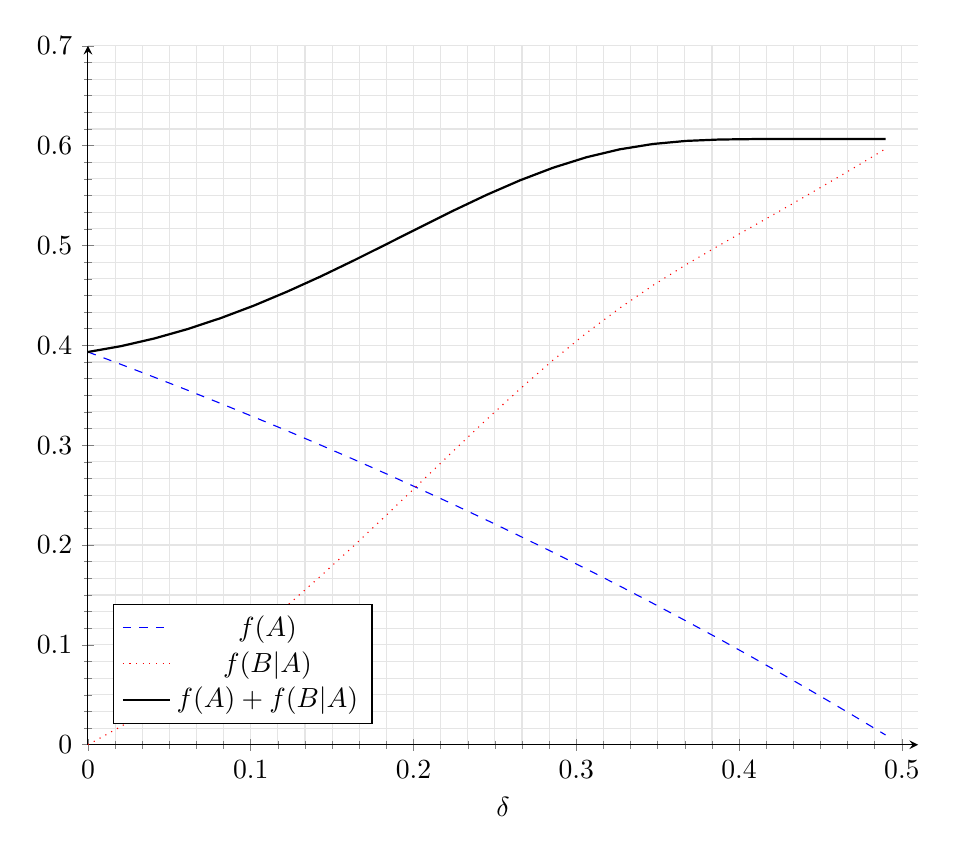
\begin{tikzpicture}
\begin{axis}[
	width=\textwidth
	,domain=0:0.49
	,ymax=.7
	,xmax=.51
	,xlabel=$\delta$
	,xtick distance=0.1
	,ytick distance=0.1
	,axis lines=left
	,grid=both
	,grid style={
		draw=gray!20
	}
	,minor tick num=5
	,legend pos=south west
	,legend entries={
		$f(A)$
		,$f(B|A)$
		,$f(A) + f(B|A)$
	}
]
  \addplot[blue, dashed, thin]{1-exp(-(0.5-x))};
  \addplot[red, dotted, thin]{(1 - exp(-(4*x/(1-2*x)))) * (exp(-1/2) - 1 + exp(-(1/2-x)))};
  \addplot[black, thick]{1-exp(-(0.5-x)) + (1 - exp(-(4*x/(1-2*x)))) * (exp(-1/2) - 1 + exp(-(1/2-x)))};
\end{axis}
\end{tikzpicture}
\end{figure}

\paragraph{Upper Bound}
In \cite{khuller1999budgeted} it is claimed that the upper bound on the approximation ratio
of the modified greedy algorithm is at most 0.44, but no explicit instance was given to 
support this claim and we could not reproduce such an example.
Here we give a simple example that bound the approximation ratio from above by $1-e^{-2/3}$, 
leaving a gap between the lower and upper bounds.
Consider an instance of the budgeted maximum coverage problem where the optimal cover consists
of 3 disjoint subsets, $S_1, S_2, S_3$ each cover exactly third of the ground set. 
In this example we assume a uniform weight function, and suppose the cost of each subsets of 
the optimal solution is $1/3$. We now describe the subsets that the modified greedy algorithm
may choose. Consider $k + 1$ disjoint subsets $T_1, \dots, T_{k + 1}$ where $c(T_i) = 2/3k$, 
where subset $T_i$ covers $\frac{2}{3k}(1-\frac{2}{3k})^i$ fraction of the ground set and for
every $i$ it holds that $|T_i \cap S_1| = |T_i \cap S_2| = |T_i \cap S_3|$.
One can verify that the modified greedy algorithm might chose those sets leaving no budget for
any of the optimal subsets. As $k$ approaches infinity the total value of those sets approches
$1-e^{-2/3}$. 



  